% Based on:
% THIS IS SIGPROC-SP.TEX - VERSION 3.1
% WORKS WITH V3.2SP OF ACM_PROC_ARTICLE-SP.CLS
% APRIL 2009
%
% Edited with TeXStudio 2.8.8

\documentclass{acm_proc_article-sp}

% For code listings:
\usepackage{listings}
\usepackage{color}
\definecolor{dkgreen}{rgb}{0,0.6,0}
\definecolor{gray}{rgb}{0.5,0.5,0.5}
\definecolor{mauve}{rgb}{0.58,0,0.82}
\lstset{frame=tb,
	language=Sparql,
	aboveskip=3mm,
	belowskip=3mm,
	showstringspaces=false,
	columns=flexible,
	basicstyle={\small\ttfamily},
	numbers=none,
	numberstyle=\tiny\color{gray},
	keywordstyle=\color{blue},
	commentstyle=\color{dkgreen},
	stringstyle=\color{mauve},
	breaklines=true,
	breakatwhitespace=true,
	tabsize=3
}

% For tables:
\usepackage{booktabs}
\newcommand{\head}[1]{\textnormal{\textbf{#1}}}

\usepackage{array}
\newcolumntype{L}{>{\centering\arraybackslash}m{3cm}}

\begin{document}

\title{Semantic Exploration of Native American Ethnobotany}

\subtitle{
	\textit{Submitted as required engineering project report}\\
	\textbf{Indiana University ILS-Z636: Data Semantics, Fall 2014}\\
	\textbf{Professor Ying Ding}\\
}


\numberofauthors{2}

\author{
%1st author
\alignauthor
Stefan M. Furrer\\
       \affaddr{Indiana University}\\
       \affaddr{Bloomington, IN}\\
       \email{stfurrer@indiana.edu}
%2nd author
\alignauthor
Jeremy J. Yang\\
       \affaddr{Indiana University}\\
       \affaddr{Bloomington, IN}\\
       \email{jejyang@indiana.edu}
}


\maketitle
\begin{abstract}
A semantic knowledge base and web interface was developed for the exploration of Native American Ethnobotany. We used the Jena API and toolkit and modern W3C semantic web standards including RDF, Turtle and Sparql to model the data. Public ontologies were used in compliance with Linked Open Data (LOD) principles. NCBI Taxonomy\footnote{http://www.ncbi.nlm.nih.gov/taxonomy} and MeSH\footnote{http://www.ncbi.nlm.nih.gov/mesh} controlled vocabulary were used as well.  
 
\end{abstract}

% A category with the (minimum) three required fields
\category{H.4}{Information Systems Applications}{Miscellaneous}

\keywords{Semantic web, RDF, Sparql, ethnobotany, library science, informatics, data science, cultural heritage}

\section{Introduction}
Ethnobotany studies both the plants and their relationship to a culture, in this case, indigenous people of North America. In addition to its value to social science, it is often the case that cultural heritage knowledge\cite{Hyvonen:cult} can provide unique insights for the natural sciences, for example, traditional medicines. Native American Ethnobotany\footnote{https://en.wikipedia.org/wiki/Native\_American\_ethnobotany} has been studied and cataloged by various scholars\cite{moerman:native} including for an online database at U. Michigan - Dearborn\footnote{http://herb.umd.umich.edu/}, which was first released as an electronic database in 1977. Cultural heritage knowlege in general, and ethnobotany in particular, is highly contextual. In other words, to correctly represent and apply knowledge across cultures requires sufficient understanding of those cultures, especially their languages and modes of communication.  This can be considered metadata, but a deeper understanding of metadata leads us directly to concepts and methods of data semantics technologies. Learning from cultural heritage is a type of deep semantic translation.  This project applies semantic methods and technologies to the ethnobotanical knowledge learned and propagated over the  millenia by Native Americans.  However, the breadth of this project is limited by the scope of this class project.


\section{Theory and Background}
This project and the Data Semantics course itself are based on several foundational disciplines including: library and computer science, logic, and linguistics\cite{Allemang:swftwo}.  This fusion is generally reflected in the new fields of "informatics" and "data science." The terminology in part reflects a change of emphasis, toward the data, information and knowledge and its representation, semantics and processing. In its highest aspiration, knowledge processing is synonymous with intelligence. With this very abstract background, the research question driven by this project is whether empirical knowledge of Native American ethnobotany can be represented and queried via semantic methods, and whether such methods can yield advantages. By definition, ethnobotany data is empirical, based on oral traditions and teachings, culturally propagated knowledge, accompanied by strong belief and contrasting sharply with modern laboratory results with scant data but mechanistic implications. A systematic evaluation and comparison of indigenous pharmacopoeias is of great interest for natural product discovery in the pharmaceutical industry as well as to contribute to improved health care in marginalized regions. The cultural and linguistic diversity represented in the numerous collections of ethnobotanical accounts worldwide presents an unique opportunity for the vision of the Semantic Web, where heterogenous data can be queried and different services are integrated \cite{bizer:2009}. 

\subsection{Related Work}
Medicinal plants are an important component of indigenous medicine systems since ancient time and often perceived as a cultural heritage. Major research efforts in collecting ethnobotanical reports have resulted in vast amount of information about medicinal plants and cultures \cite{Heinrich:2006}. With having often a cultural or regional focus, such ethnobotanical databases lack uniformity and interlinkability \cite{Ningthoujam:2012}, both major efforts of the Linked Open Data\footnote{http://www.w3.org/wiki/SweoIG/TaskForces/CommunityProjects/LinkingOpenData} initiative. The integration of ontologies, Semantic Web languages (XML, RDF and OWL) or taxonomic standards that would enable an automated data exchange and search federation, has been discussed for particular cultural collections \cite{KamsuFoguem:2013}, \cite{Mustaffa:2012}, \cite{Zhou:2004}, but is not consistently implemented on a global scale. One of the few examples of Semantic Web efforts in the area of traditional medicine is RDF-TCM\footnote{http://www.open-biomed.org.uk/rdf-tcm/ (SPARQL endpoints not operational 12/12/2014)}, containing information on over 800 herbs used in Traditional Chinese Medicine (TCM) and links to  DBpedia\footnote{http://dbpedia.org/} and DailyMed\footnote{http://dailymed.nlm.nih.gov/dailymed/} among others \cite{zhao:2010}. 

\begin{figure}
	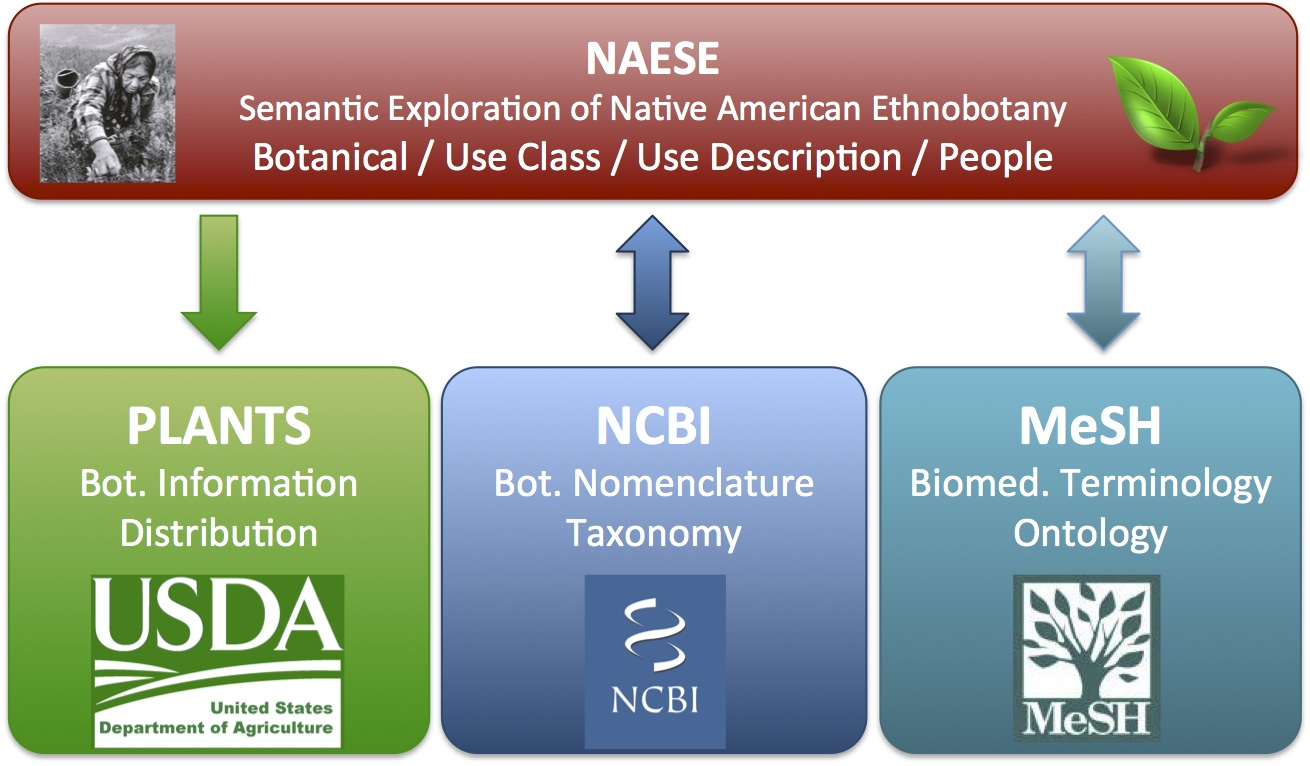
\includegraphics[width=\linewidth]{NAESE_architecture}
	\caption{Naese data sources and connections.}
	\label{fig:NaeseSources}
\end{figure}

\section{Datasets}
The database of Native American Ethnobotany focuses on the traditional usage of plants by Native American people, as medicines but also other purposes, such as food \cite{moerman:analysis},\cite{moerman:native}. The data was accessed from the Native American Ethnobotany database on September 13, 2014 through a series of genera specific searches and the data processed into a tabular format. For the purpose of this project, only information on ethnomedicinal plant knowledge was considered, or 25'311 different usages for 3'074 kinds of plants (species, subspecies, varieties), ranging from cold remedies and analgesics to witchcraft uses. 

\subsection{Data Standards and Annotation}
The heterogeneity of ethnobotanical data, amplified by cultural and linguistic differences, together with a lack of standard terminology are adding complexity to the integration and interlinking with other information resources \cite{Cheung:TCM}. The utilization of a common terminology to describe a medicinal plant and its usage are prerequisites for developing a system that allows automated data exchange. In addition to plant usage categories assigned in Native American Ethnobotany, the particular bits of information about the utilization of plants were indexed using Medical Subject Headings (MeSH) vocabulary \cite{Bodenreider:UMLS}. The NLM Medical Text Indexer (MTI)\footnote{http://skr.nlm.nih.gov/batch-mode/mti.shtml} was utilized to efficiently and consistently annotate the detailed plant usage indications with an ontology based biomedical terminology \cite{Mork:MTI}. Out of a total of 19'382 unique medicinal plant use indications, 727 or 4\% resulted in errors and could not be annotated with corresponding MeSH terms. A manual evaluation of the selected records indicated an excellent and correct indexing, although in some cases word sense ambiguity lead to contextually incorrect annotation, such as the tagging of "(plant) gum" with "Gingiva" (MeSH: D005881) \cite{Stevenson:Disambiguation}.

Only few databases emphasize the application of a standardized identification and taxonomy for botanicals and synonyms, superfluous, ambiguous or misspelled taxon names result in mismatched records. The Taxonomic Name Resolution Service (TNRS)\footnote{http://tnrs.iplantcollaborative.org} \cite{Pubmed:23324024} provides a botanical name parsing and fuzzy matching against multiple reference taxonomies, including the NCBI taxonomy\footnote{http://www.ncbi.nlm.nih.gov/taxonomy/}
\cite{Sayers:NCBITax1},\cite{Benson:NCBITax2} and USDA PLANTS\footnote{http://plants.usda.gov} database. Careful manual curation of the taxonomy matching results was performed to enable a correct and accurate alignment with the taxonomies if possible. Due to different taxonomic coverages, an assignment of to the exact subspecies or species was not possible in every case. Missing botanical information resulted in assigning to a higher taxonomic level. For the 3'074 different botanicals, the taxonomic alignment resulted in 114 different subspecies/variety, 2'230 species and 348 unique genus.


\begin{table}
	\centering
	\caption{Datasets used and number of unique entities represented in project}
	\begin{tabular}{|c|c|c|c|}
		\toprule[1.5pt]
		\head{Name} & \head{Publisher} & \head{Entities}\\
		\midrule
		Native American Ethnobotany & U. Michigan & 25'311 \\
		Taxonomy & NCBI & 2'692 \\ 
		MeSH & NLM & 1'442 \\
		PLANTS & USDA & 2'921 \\ 
		\bottomrule[1.5pt]
		\end{tabular}
\end{table}

\subsection{Knowledge Representation: Modeling the Data}
The ethnobotanical data and its biomedical and taxonomic annotation was organized and converted into a knowledge representation of the domain. The raw data files were processed, combined, and converted to RDF, serialized as RDF-XML and TTL formats, using OpenRefine\footnote{http://openrefine.org}. An RDF data skeleton was defined according to domain concepts and predetermined search scenarios. Throughout the development of the data skeleton, care was taken to identify concepts (or classes) of prominent dictionaries, such as Dublin Core Metadata Intiative (DCMI)\footnote{http://dublincore.org/documents/dcmi-terms/} that can be reused, such as dc:title. The knowledge base skeleton was structured for a botanical to be identified by its botanical and common name, as well as taxonomy links. Each botanical is a member of a certain use description that references the corresponding biomedical terminology, usage category as well as the Native People for which the use was reported. The NCBI taxonomy and MeSH terminology were integrated through interlinking to the URI's of the RDF representations of the corresponding datasets in bio2rdf\footnote{http://bio2rdf.org} \cite{Belleau:2008}. Since the USDA PLANTS taxonomy is not available in RDF format, the knowledge base was populated with the corresponding ID instead of referencing these resources (using URI).

\begin{figure}
	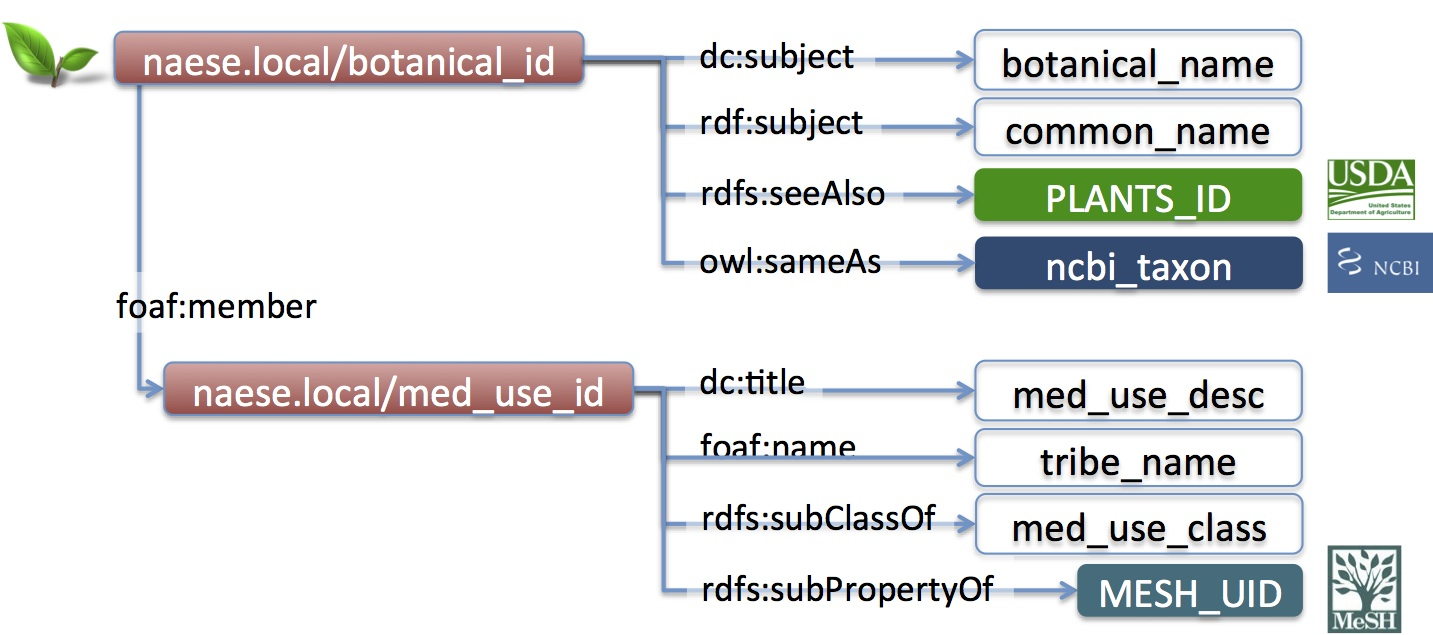
\includegraphics[width=\linewidth]{RDF_skeleton_naese}
	\caption{Naese knowledge base skeleton.}
	\label{fig:NaeseSkeleton}
\end{figure}

\section{Engineering Project: web application Naese}
The purpose of the web app in this project is to demonstrate the semantic data methods which are the central aim. An effective web app not only provides end users with a usable interface, but can accelerate and improve development by providing a convenient testing tool. Web apps can be conveniently deployed over heterogeneous networks for distributed audiences. This was an important capability for our distributed team of distance students, located in Ohio and New Mexico, for a course based in Indiana.


\subsection{Methods and Tools}

\begin{figure*}[t]
\centering
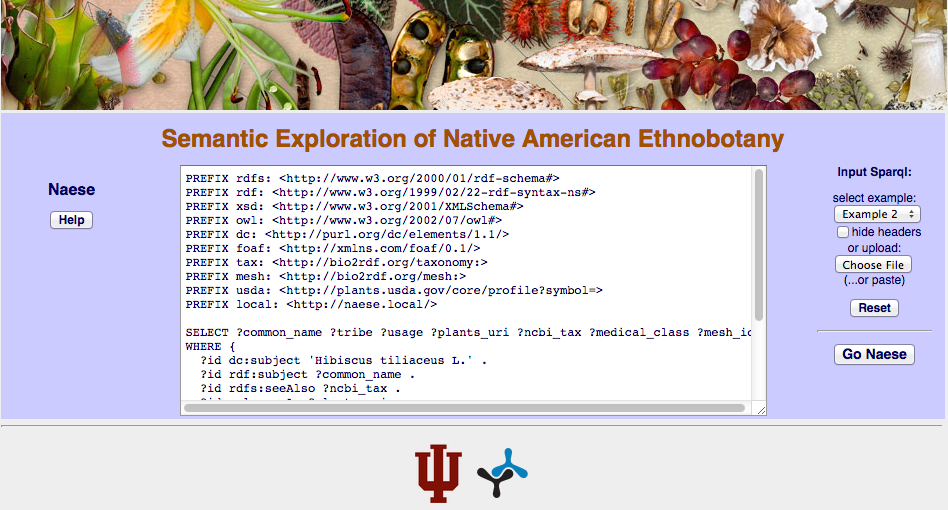
\includegraphics[width=0.8\linewidth]{Naese_demo_04}
\caption[Naese web app]{Naese web app with example query loaded.}
\label{fig:Naese_demo_04}
\end{figure*}
 
Naese was implemented as a Java Enterprise web app and deployed via WAR file using Tomcat. Naese was built using Jena 2.12.0\footnote{http://jena.apache.org/}. Jena is described as "A free and open source Java framework for building Semantic Web and Linked Data applications". In this project, several Jena methods and tools were employed, including the Java API and command-line applications.

With Jena there are several options for dataset storage. To implement a self-contained WAR, for convenient and robust web app deployment, the RDF data file (RDF-XML) was included and an in-memory datastore is initialized on web app deployment. This improves performance at runtime by avoiding overhead, by pre-loading data.  Jena can also be used to deploy a Sparql endpoint (service) using Fuseki\footnote{http://jena.apache.org/documentation/serving\_data/}.  Also Jena TDB\footnote{https://jena.apache.org/documentation/tdb/} can be used to implement persistent storage from an input file, and support read/write access. Sparql endpoint deployment also supports LOD standards and applications from generic Sparql clients, including federated queries.

\subsection{Case Study: Example of Pain Remedies}
The benefits of using standardized terminology and ontologies is highlighted for instance, on pain remedies utilized by Native American people. Querying the dataset for botanicals associated with the MeSH term "Pain" (mesh: D010146), does recruit botanicals from many different use classification, including analgesic, dermatological and gynecological uses, among others. A close look at the use descriptions of these botanicals does highlight the value of the controlled terminology of MeSH and the MTI tagger, as not only "pain", but also synonyms of the term, such as "aches" or "sore" are classified alike. The ranking of these botanicals by their most frequent use, in terms of number of tribes associated with the botanical and "pain" MeSH term, products a significance ranking or cross-cultural validation, biased by a botanicals geographic distribution. \textit{Acorus calamus}, also called Sweet Flag or Calamus, is one of the top ranked species and the analgesic effect of ethanolic root extracts has been studied in mice and significant activity has been observed \cite{Khan:2012}.

\subsection{Example Queries, Use Cases}
One approach to data resource design is to begin with the desired queries, that is, the questions which should be answerable, and design the system to fulfill those design requirements. Whether this approach is used or not, typically, since development often iterates cyclically, the effect will be the same: databases are about answering questions, so good example questions are essential, and in many ways define the project. Output is excerpted below due to space limitations. Full queries and output is included in supplementary materials.

\textbf{Sparql headers:}
\begin{lstlisting}
PREFIX rdfs: <http://www.w3.org/2000/01/rdf-schema#>
PREFIX foaf: <http://xmlns.com/foaf/0.1/>
PREFIX owl: <http://www.w3.org/2002/07/owl#>
PREFIX xsd: <http://www.w3.org/2001/XMLSchema#>
PREFIX rdf: <http://www.w3.org/1999/02/22-rdf-syntax-ns#>
PREFIX tax: <http://bio2rdf.org/taxonomy:>
PREFIX voc: <http://bio2rdf.org/taxonomy_vocabulary:>
PREFIX mesh: <http://bio2rdf.org/mesh:>
PREFIX usda: <http://plants.usda.gov/core/profile?symbol=>
PREFIX local: <http://naese.local/>
\end{lstlisting}

\textbf{Example query: Toothache remedies}
Find all botanicals used for toothache. Note that toothache remedies are a subclass of analgesics. This illustrates a fundamental advantage of semantic methods, as the query could easily be broadened. Likewise, a species can be associated with related species via taxonomy subclasses.
\begin{lstlisting}
SELECT DISTINCT ?id ?species ?tribe ?title ?subClassOf
WHERE {
  FILTER (regex(?subClassOf, 'Toothache', 'i')) .
  ?usage rdfs:subClassOf ?subClassOf . 
  ?usage foaf:name ?tribe . 
  ?usage dc:title ?title . 
  ?id foaf:member ?usage . 
  ?id dc:subject ?species .
}
ORDER BY ?species ?tribe
\end{lstlisting}


\begin{table}[h]
	\centering
	\caption{Toothache query output (partial)}
	\begin{tabular}{|L|c|}
		\hline
		\head{species} & \head{tribe} \\
		\hline
\texttt{Aesculus californica} & \texttt{Mendocino} \\
\texttt{Cephalanthus occidentalis L.} & \texttt{Cherokee} \\
\texttt{Cephalanthus occidentalis L.} & \texttt{Choctaw} \\
\texttt{Cephalanthus occidentalis L.} & \texttt{Kiowa} \\
\texttt{Cephalanthus occidentalis L.} & \texttt{Thompson} \\
\texttt{Juglans nigra L.} & \texttt{Cherokee} \\
\texttt{Juglans nigra L.} & \texttt{Choctaw} \\
\texttt{Juglans nigra L.} & \texttt{Thompson} \\
\texttt{Salix sp.} & \texttt{Cherokee} \\
\texttt{Salix sp.} & \texttt{Choctaw} \\
\texttt{Salix sp.} & \texttt{Kiowa} \\
\texttt{Salix sp.} & \texttt{Thompson} \\
\texttt{Sambucus racemosa L.} & \texttt{Okanagon} \\
\texttt{Sambucus racemosa L.} & \texttt{Thompson} \\
\texttt{Shepherdia rotundifolia Parry} & \texttt{Navajo, Kayenta} \\
\texttt{Zanthoxylum americanum P. Mill.} & \texttt{Iroquois} \\
\hline
	\end{tabular}
\end{table}

\textbf{Example query: Plant name}
Search for botanical by official name (Latin). Show common name, tribe, usage, and external linking IDs.
\begin{lstlisting}
SELECT ?common_name ?tribe ?title ?medical_class ?plants_uri ?ncbi_tax ?mesh_id
WHERE {
  ?id dc:subject 'Hibiscus tiliaceus L.' .
  ?id rdf:subject ?common_name . 
  ?id rdfs:seeAlso ?ncbi_tax . 
  ?id owl:sameAs ?plants_uri . 
  ?id foaf:member ?usage . 
  ?usage dc:title ?title . 
  ?usage foaf:name ?tribe . 
  ?usage rdfs:subClassOf ?medical_class . 
  ?usage rdfs:subPropertyOf ?mesh_id .
}
\end{lstlisting}

\begin{table}[h]
	\centering
	\caption{Plant name query output (partial)}
	\begin{tabular}{|r|L|}
		\hline
		\head{common\_name} & \texttt{Sea Hibiscus}  \\
		\cline{2-2}
		\head{tribe} & \texttt{Hawaiian} \\
		\cline{2-2}
		\head{medical\_class} & \texttt{Pulmonary Aid} \\
		\cline{2-2}
		\head{title} & \texttt{Bark and other plants crushed, water added, strained and resulting liquid taken for congested chest} \\
		\hline
	\end{tabular}
\end{table}



\begin{figure}[h]
\centering
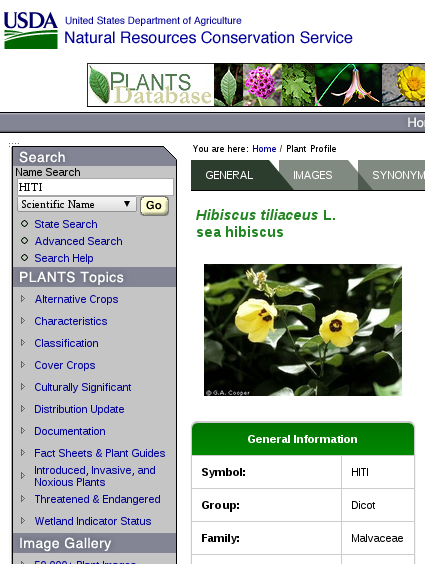
\includegraphics[width=1.0\linewidth]{USDA_Plants_HITI}
\caption[USDA Plants: HITI]{USDA Plants page for Hibiscus tiliaceus L., symbol HITI\footnote{http://plants.usda.gov/core/profile?symbol=HITI}.}
\label{fig:USDA_Plants_HITI}
\end{figure}


\textbf{Example query: Federated query}
Use SERVICE sub-query for remote endpoint access, to include linked MeSH terms and descriptions. \textit{(Not supported by Naese web app, due to Jena API limitations.)}
\begin{lstlisting}
SELECT ?naese_id ?subject ?mesh_id ?mesh_term ?mesh_description
WHERE {  
  ?naese_id dc:subject 'Hibiscus tiliaceus L.' .
  ?naese_id rdf:subject ?subject . 
  ?naese_id rdfs:subPropertyOf ?mesh_id .
  ?mesh_id rdf:type local:mesh_UID
  SERVICE <http://mesh.bio2rdf.org/sparql>
  {
    SELECT ?mesh_id ?mesh_term ?mesh_description
    WHERE {
      ?mesh_id voc:mesh-heading ?mesh_term . 
      ?mesh_id voc:mesh-scope-note ?mesh_description
    }
  }
}
\end{lstlisting}

\textbf{Example query: Bio2RDF MeSH endpoint}
Using a generic Sparql client, fetch by MeSH ID. In effect this implements a manual federated search.
\begin{lstlisting}
$ sparql_query.py --url http://mesh.bio2rdf.org/sparql --rqfile mesh_remote.rq --fmt TTL
@prefix res: <http://www.w3.org/2005/sparql-results#> .
@prefix rdf: <http://www.w3.org/1999/02/22-rdf-syntax-ns#> .
_:_ a res:ResultSet .
_:_ res:resultVariable "MeSH_Term" , "MeSH_Description" .
_:_ res:solution [
res:binding [ res:variable "MeSH_Term" ; res:value "Plant Roots" ] ;
res:binding [ res:variable "MeSH_Description" ; res:value "The usually underground portions of a plant that serve as support, store food, and through which water and mineral nutrients enter the plant. (From American Heritage Dictionary, 1982; Concise Dictionary of Biology, 1990)" ] ] .

sparql_query.py: input file: mesh_remote.rq
\end{lstlisting}

\section{Evaluation}
The usability and functionality of the Naese web app was evaluated by the project team in the context of molecular discovery science.  The simple textual input for Sparql does not provide GUI features for editing, but the example queries do provide multiple useful, editable templates. The output is simple text, and could be improved by formatting and alternate modes, especially downloadable files. Currently there is no support for federated queries (e.g. via SERVICE), so this could be a major enhancement, but would require re-architecture to employ a Sparql endpoint instead of embedded Jena TDB triple store. This would also enable rule based queries, utilizing utilizing the MeSH ontology and NCBI taxonomic classification. Further enrichment of the data set, for example through reconciliation with DBpedia, as well as integration of other ethnobotanical data sources, such as Plants for a Future\footnote{http://www.pfaf.org} would allow searches across cultural and regional collections. A refinement of the data model and further utilization of existing dictionaries, such as skos:altLabel for the "common name" and a local resource for the tribe (tribe\_id).

\section{Conclusions}
A data model was developed to represent and process knowledge about Native American ethnobotany. This data model was implemented using Jena and deployed as a JEE web app for testing and usage. A range of queries which demonstrate a range of capabilities were developed and tested. The advantages of semantics are conferred and illustrated by subclass relationships such as toothache-remedies as a subclass of analgesics, and taxonomy subclass relationships to facilitate phylogenetic or chemotaxonomic similarity exploration.


\section{Acknowledgments}
The authors would like to thank the instructor, Prof. Ying Ding, and assistant instructors of Data Semantics ILS-Z636, for their efforts and support, and especially for supporting the participation of distance learners through online education technologies, another very promising, rapidly evolving area.

\section{Author Contributions}
SF conceived the project, developed the data model, acquired and pre-processed the data using OpenRefine, producing RDF in RDF-XML and TTL formats, and developed use-cases via example Sparql queries. JY developed Jena API code, Jena TDB command-line workflows, and Jena Fuseki tools, to deploy the dataset via TDB, as a Sparql endpoint, and via Java Enterprise web app, deployed via WAR file. SF and JY cooperatively and equally authored the report, tested and revised Sparql queries and use cases.

% The following two commands are all you need in the initial runs of your .tex file to
% produce the bibliography for the citations in your paper.
\bibliographystyle{abbrv}
\bibliography{NativeAmericanEthnobotany}  % NativeAmericanEthnobotany.bib should exist

\begin{table}[h]
	\centering
	\begin{tabular}[width=\linewidth]{|L|}
		\hline
	This document is compliant with ACM Proceedings format\footnote{http://www.acm.org/sigs/publications/proceedings-templates}, and was authored using TeXstudio\footnote{http://texstudio.sourceforge.net/}. \\
		\hline 
	\end{tabular}
\end{table}



\end{document}
